\vfill\null\columnbreak
\section{Systemanalyse im Zeitbereich}
Für ein lineares zeitinvariantes SISO System gilt:
    \subsection{Allgemeine Lösung}
        \[ \dot{x}(t) = A \cdot x(t) + b \cdot u(t) \hspace{4mm} A \in\mathbb{R}^{n \times n}, b \in\mathbb{R}^{n \times 1} \]
        \[ y(t) = c \cdot x(t) + d \cdot u(t) \hspace{4mm} c \in\mathbb{R}^{1 \times n}, d \in\mathbb{R}\]
        \[x(0) = x_0\]
        
        die allgemeine Lösung der Zustandsgrösse $x(t)$ ist gegeben als: 
        \[ x(t) = e^{A\cdot t} \cdot x_0 + \int_0^t e^{A\cdot(t-p)}\cdot b \cdot u(p)dp\]
        
        Setzt man die allgemeine Lösung in die Gleichung der Ausgangsgrösse y(t) ein, erhält man die Superposition dreier Grössen:
        
         \[ y(t) = \underbrace{c\cdot e^{A\cdot t} \cdot x_0}_\text{I} + c \underbrace{\cdot \int_0^t e^{A\cdot(t-p)}\cdot b \cdot u(p)dp}_\text{II} + \underbrace{d\cdot u(t)}_\text{III}\]
         
         Die \textbf{natürliche Antwort} des Systems ($I$) ist unabhängig von der Eingangsgrösse $u$. Der Eingang u trägt einerseits zum Beitrag der \textbf{Systemdynamik} ($II$) bei, und andererseits zum \textbf{Feedthrough Term} ($III$)
    \subsection{Stabilitätseigenschaften}
        Um die Stabilität eines Systems zu bestimmen betrachtet man die natürliche Antwort des Systems ($u(t)=0$). Da die Zustandsgleichungen im Allgemeinen gekoppelt sind führt man eine Koordinatentransformation durch.
        \[\Tilde{x}=V^{-1}\cdot e^{A\cdot t}\cdot V \cdot\Tilde{x}(0)=e^{\Tilde{A}\cdot t}\cdot\Tilde{x}(0)\]
        \[\Tilde{x}=
        \begin{bmatrix}
            e^{\lambda_1\cdot t}    & 0                     & \dots & 0 \\
            0                       & e^{\lambda_2\cdot t}  & \dots & 0 \\
            \vdots                  & \ddots                & \ddots & \vdots\\
            0                       & \dots    &\dots             & e^{\lambda_n\cdot t}
        \end{bmatrix}
        \Tilde{x_0}=
        \begin{bmatrix}
            e^{\lambda_1\cdot t}\cdot\Tilde{x}_{0,1}  \\
            e^{\lambda_2\cdot t}\cdot\Tilde{x}_{0,2} \\
            \vdots  \\
            e^{\lambda_n\cdot t}\cdot\Tilde{x}_{0,n} 
        \end{bmatrix}
        \]
        wobei $\lambda_i$ die Eigenwerte von $A$ (resp. $a^{-1}$) sind. Da die EW generell Komplex sind ($\lambda_i=\sigma_i+j\omega_i$) kann man die obige Gleichung auch umschreiben.
        \[
        \begin{bmatrix}
            e^{\lambda_1\cdot t}\cdot\Tilde{x}_{0,1}  \\
            e^{\lambda_2\cdot t}\cdot\Tilde{x}_{0,2} \\
            \vdots  \\
            e^{\lambda_n\cdot t}\cdot\Tilde{x}_{0,n} 
        \end{bmatrix}
        =
        \begin{bmatrix}
            e^{\sigma_1\cdot t}\cdot\left(cos(\omega_1t)+j\cdot sin(\omega_1t)\right)\cdot\Tilde{x}_{0,1}  \\
            e^{\sigma_2\cdot t}\cdot\left(cos(\omega_2t)+j\cdot sin(\omega_2t)\right)\cdot\Tilde{x}_{0,2} \\
            \vdots  \\
            e^{\sigma_n\cdot t}\cdot\left(cos(\omega_nt)+j\cdot sin(\omega_nt)\right)\cdot\Tilde{x}_{0,n} 
        \end{bmatrix}
        \]
        \begin{center}
            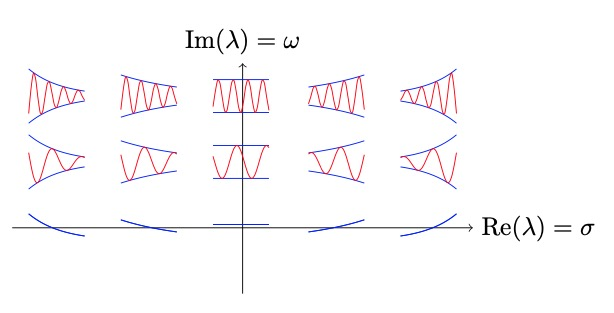
\includegraphics[width=0.8\linewidth]{03/sysantwort.jpg}
            %Symmetrisch um $\textrm{Re}(\lambda)=\sigma$-Achse.
        \end{center}
        
    \subsection{Lyapunov Stabilität}
        Stabilität nach Lyapunov erlaubt die Stabilitätsanalyse von Gleichgewichstpunkten (GGWP) von linearen und linearisierten Systemen.\\\\
        \textbf{WICHTIG! Falls ein GGWP eines linearisierten Systems Eigenwerte mit $\sigma_i=0$ hat, lässt sich keine Aussage über die Stabilität dieses GGWP des nichtlinearen Systems machen.}
        \begin{enumerate}
            \item \textbf{Asymptotisch stabil:} $\displaystyle\lim_{t\to\infty}\Vert x(t)\Vert = 0 $, falls alle EW $\textrm{Re}(\lambda_i)<0$.
            \item \textbf{Stabil:} ($\Vert x(t)\Vert<\infty \forall t \in[0,\infty]$), falls mehrere EW $\textrm{Re}(\lambda_k)=0$ und kein EW $\textrm{Re}(\lambda_i)\ngtr 0$.
            \item \textbf{Instabil:} $\displaystyle\lim_{t\to\infty}\Vert x(t)\Vert = \infty$ falls mindestens ein EW $\textrm{Re}(\lambda_i)>0$.
        \end{enumerate}{}
        \subsubsection{Bsp}
            \[m\Ddot{x}=-c_D\dot{x}-k_Fx+u(t)\]
            \[\Rightarrow \Ddot{x}=
                \begin{bmatrix}
                    0   &   1\\
                    -k_F/m  &   -c_D/m\\
                \end{bmatrix}
                \begin{bmatrix}
                    x_1\\
                    x_2\\
                \end{bmatrix}
                +
                \begin{bmatrix}
                0\\
                1\\
                \end{bmatrix}
                u(t)
            \]
            \[\textrm{Det}(A-\lambda\mathbb{I}) \Rightarrow \lambda_i=-\frac{c_D}{2m}\pm \sqrt{\frac{c_D^2}{4m^2}-\frac{k_F}{m}}\]
            
            \begin{enumerate}
                \item $\displaystyle \frac{c_D^2}{4m^2}-\frac{k_F}{m}\geqslant 0
                \Leftrightarrow c_D^2 \geqslant 4k_Fm \Rightarrow\boxed{\sigma_i<0,\omega_i=0}$
                
                Falls der Dämpfer relativ zur Feder und zur Masse genug stark ist, sind alle EW reellwertig negativ. Dh, das System konvergiert ohne Oszillation zum GGWP. \boxed{\textrm{\textit{Asymptotisch stabil} nach Lyapunov.}}
                \item $\displaystyle c_D^2 \leqslant 4k_Fm \Rightarrow\boxed{\sigma_i<0,\omega_i\neq0}$
                \\Falls der Dämpfer schwach ist, werden die EW komplex, mit negativem Realteil. Dh, das System oszilliert um den GGWP mit abnehmender Amplitude. \boxed{\textrm{\textit{Asymptotisch stabil} nach Lyapunov.}}
                \item $\displaystyle c_D=0 \Rightarrow\boxed{\sigma_i=0,\omega_i\neq0}$
                \\Falls kein Dämpfer im System vorhanden ist, werden alle Eigenwerte Komplex mit Realteil $\sigma_i=0$. Das System oszilliert für immer um den GGWP.
                \boxed{\textrm{\textit{Stabil} nach Lyapunov.}}
                \item $\displaystyle k_F=0 \Rightarrow\boxed{\lambda_1=0,\sigma_2<0,\omega_2=0}$
                \\Falls keine Feder im System ist, wird ein EW 0 und der andere wird reell negativ. Falls das System mehrmals angestossen wird, kommt es jedes mal ohne Oszillation zum Stillstand, jedoch nicht zwingend um den GGWP.
                \boxed{\textrm{\textit{Stabil} nach Lyapunov.}}

                
            \end{enumerate}
        
        \subsection{Testsignale auf Systeme erster Ordnung}
            Eingänge für Systeme erster Ordnung mit Zeitkonstante $\tau$ und Eingangsstärke $k$:
            \[\dot{x}(t) = -\frac{1}{\tau}x(t) + \frac{k}{\tau}u(t), \hspace{5mm} y(t) = x(t)\]
            \subsubsection{Impulsantwort}
                \[u(t) = \delta(t) = \begin{cases} +\infty, & t = 0, \\ 
                0, & t \neq 0 \end{cases}\]
                \textbf{Allgemeine Lösung:}
                \[y_{\delta}(t) = e^{\frac{-t}{\tau}}\cdot(x_0+\frac{k}{\tau})\]
        
                Ein Impuls ändert die Anfangsbedingung $x_0$ um $k / \tau $.
        
                $\rightarrow$ Impuls induziert eine Anfangsbedingung, System entwickelt sich von der neuen Anfangsbedingung, als ob $u(t) = 0$ wäre.
    
            \subsubsection{Sprungantwort}
%               \[ u(t) = h(t) = \begin{cases}
%               1, & t \geq 0\\
%               0, & t <0 \end{cases}\]
                \textbf{Allgemeine Lösung:}
                \[y_h(t) = e^{\frac{-t}{\tau}}\cdot x_0 + k \cdot (1-e^{\frac{-t}{\tau}}) \]
                \begin{center}
                    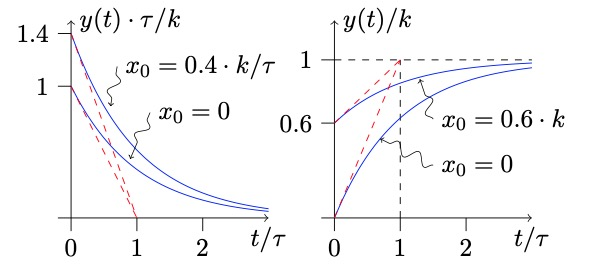
\includegraphics[width=0.7\linewidth]{03/impuls-Sprung-Antwort.jpg}\\
                    \textit{Impulsantwort links und Sprungantwort rechts.}
                \end{center}
                Die Tangente an die Impulsantwort zum Zeitpunkt $t=0$ schneidet die Zeitachse zum Zeitpunkt $t=\tau$. 
                \\Die Tangente an die Sprungantwort schneidet den Sprung $k\cdot h(t)$ auch zum Zeitpunkt $t=\tau$.
                \\Impulsantwort hat bei $t=0$ den Wert $\frac{k}{\tau}$.
                \\$\Rightarrow$ \textbf{Je kleiner $\mathbf{\tau}$, desto schneller konvergiert das System.}
            \subsubsection{Rampenantwort}
%               \[u(t)=p(t)=\begin{cases}
%               t, & t \geq 0\\
%               0, & t < 0 \end{cases}\]
                \textbf{Allgemeine Lösung:}
                \[y_p(t)=e^{-\frac{t}{\tau}}x_0+k(t+(e^{-\frac{t}{\tau}}-1)\tau)\]
            \subsubsection{Bsp}
                $\dot{x}(t)=-\frac{c_D}{m}x(t)+\frac{1}{m}u(t)\qquad\Rightarrow \tau = \frac{m}{c_D};\qquad k=\frac{\tau}{m}=\frac{1}{c_D}$
                \begin{center}
                    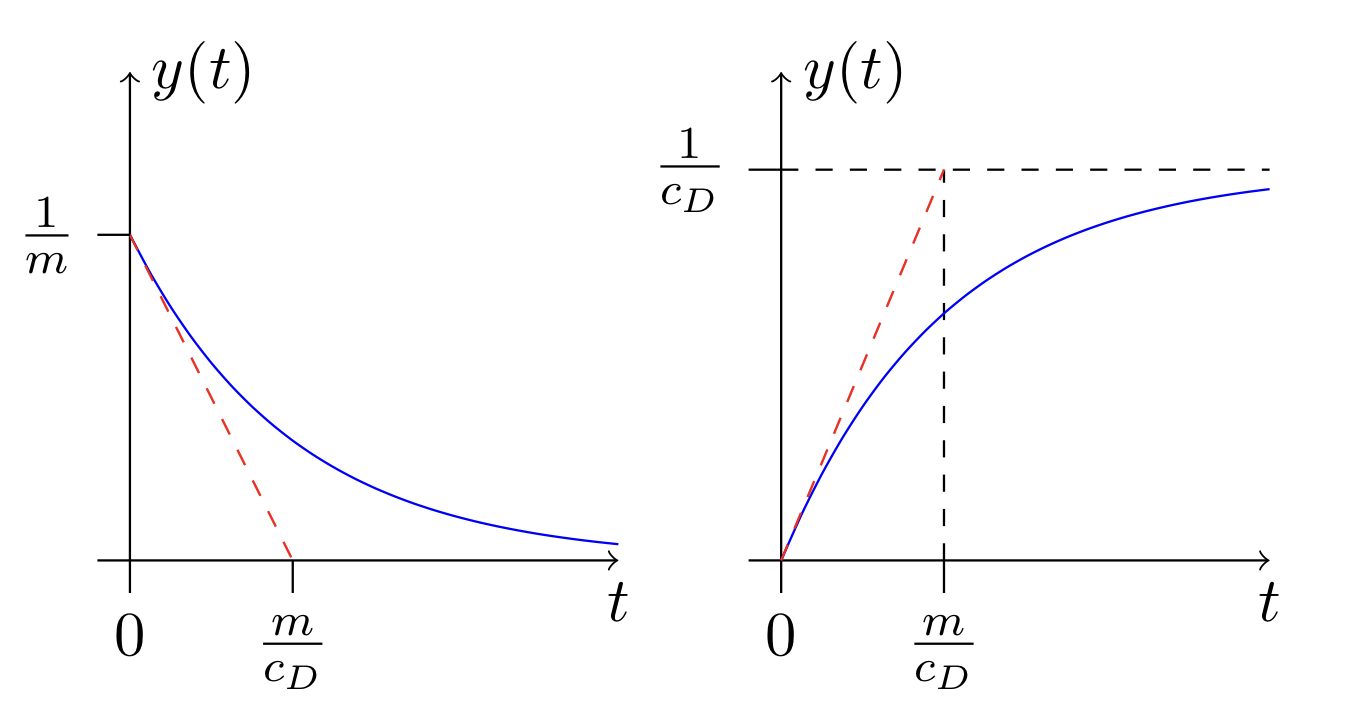
\includegraphics[width=0.75\linewidth,]{03/bsp_impuls_sprung.jpeg}
                \end{center}
                
        \subsection{Steuerbarkeit / Erreichbarkeit}
            \textbf{Steuerbar}
        falls für $x_c \in\mathbb{R}^n$ ein Eingangssignal $u(t)$ existiert, das den Zustandsvektor des Systems von $x(0) = x_c $ zum Zustand $x(\tau) = 0$ (zum Ursprung) in endlicher Zeit $\tau$ bringt. 
        
        Falls alle Punkte in $\mathbb{R}^n$ steuerbar sind, heisst das System \textit{ vollständig steuerbar}.
        Falls alle nicht-steuerbaren Zustände asymptotisch stabil sind, ist das System \textit{potentiell stabilisierbar}, 
        
        \textbf{Erreichbar} falls für $x_r \in\mathbb{R}^n$ ein Eingangssignal $u(t)$ existiert, das den Zustandsvektor des Systems von Zustand $x(t) = 0$ zum Zustand $x(\tau) = x_r$ in endlicher Zeit $\tau$ bringt.
        
        Falls alle Punkte in $\mathbb{R}^n$ erreichbar sind, heisst das System vollständig erreichbar.
        
        \textbf{WICHTIG: Für LZI Systeme sind die Teilräume der erreichbaren und steuerbaren Zustände identisch. }
        
        ein System ist vollständig steuerbar/erreichbar, wenn die \textbf{Steuerbarkeitsmatrix $\mathcal{R}$} vollen Rang hat ($\textrm{Det}(\mathcal{R})\neq0$). 
        \[\mathcal{R} = \begin{bmatrix} b, & A\cdot b, & A^2 \cdot b, & \hdots, & A^{n-1} \cdot b \end{bmatrix} \]
        \textbf{Alle Steuerbaren Zustände sind Linearkombinationen der Spalten von $\mathcal{R}$}
        
        \subsubsection{Bsp}
            \begin{center}
                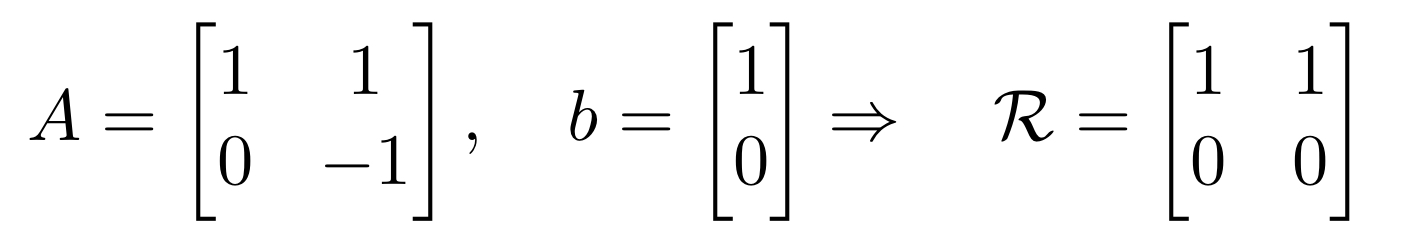
\includegraphics[width=0.7\linewidth]{03/steuerbarkeit.jpeg}\\
                $\displaystyle \textrm{Det}(\mathcal{R})\neq 0 \rightarrow$ Steuerbar
            \end{center}
            
            $\textrm{Rank}(\mathcal{R})=1<n\rightarrow$ System ist nicht vollständig erreichbar. Aus $\{A,b\}$ folgt, dass der zweite Zustand nicht direkt vom Eingang beeinflusst wird.
        \subsubsection{Stabilisierbar}
            Ein (instabiles) System ist potentiell Stabilisierbar, falls alle Zustände, die nicht steuerbar sind asymptotisch stabil sind.
            
            \textit{Remarks:}
            \\Stabilizability is a weaker condition than controllability.
            \\To stabilize an unstable system, the unstable but controllable variables have to be observable as well.
        \subsection{Beobachtbarkeit}
            Ein System ist vollständig beobachtbar, wenn man mit der Messung des Ausgangssignals $y(t), t \in [0,\tau], \tau > 0$ eindeutig auf den Anfangszustand $x(0)$ des Systems schliessen kann. 
            
            Ein LZI System ist dann vollständig beobachtbar, wenn die \textbf{Beobachtbarkeitsmatrix $\mathcal{O}$} vollen Rang hat ($\textrm{Det}(\mathcal{O})\neq0$).
            \[ \mathcal{O} = \begin{bmatrix} c \\ c \cdot A \\ c \cdot A^2 \\ \vdots \\ c \cdot A^{n-1}\end{bmatrix}\]
            
            \subsubsection{Bsp}
            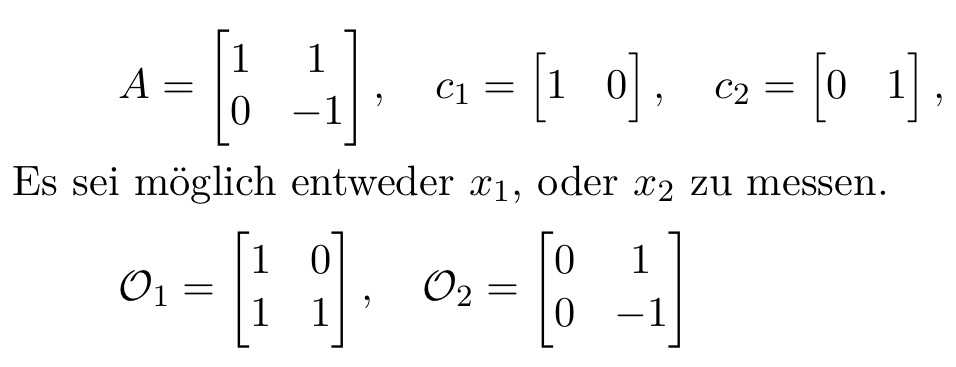
\includegraphics[width=0.8\linewidth]{03/observability.jpeg}
            \\Falls man $x_1$ misst, ist das System \textbf{vollständig beobachtbar}: $\textrm{Rank}(\mathcal{O}_1)=2$ D.h. man kann durch messen von $x_1$ auf die Anfangsbedingungen von $x_1(0)$ \& $x_2(0)$ schliessen. Falls man nur $x_2$ misst, erhält man $\textrm{Rank}(\mathcal{O}_2=1<n$. Das System ist somit nicht vollständig beobachtbar. Das ist auch in der graphischen Darstellung ersichtlich:
            \begin{center}
                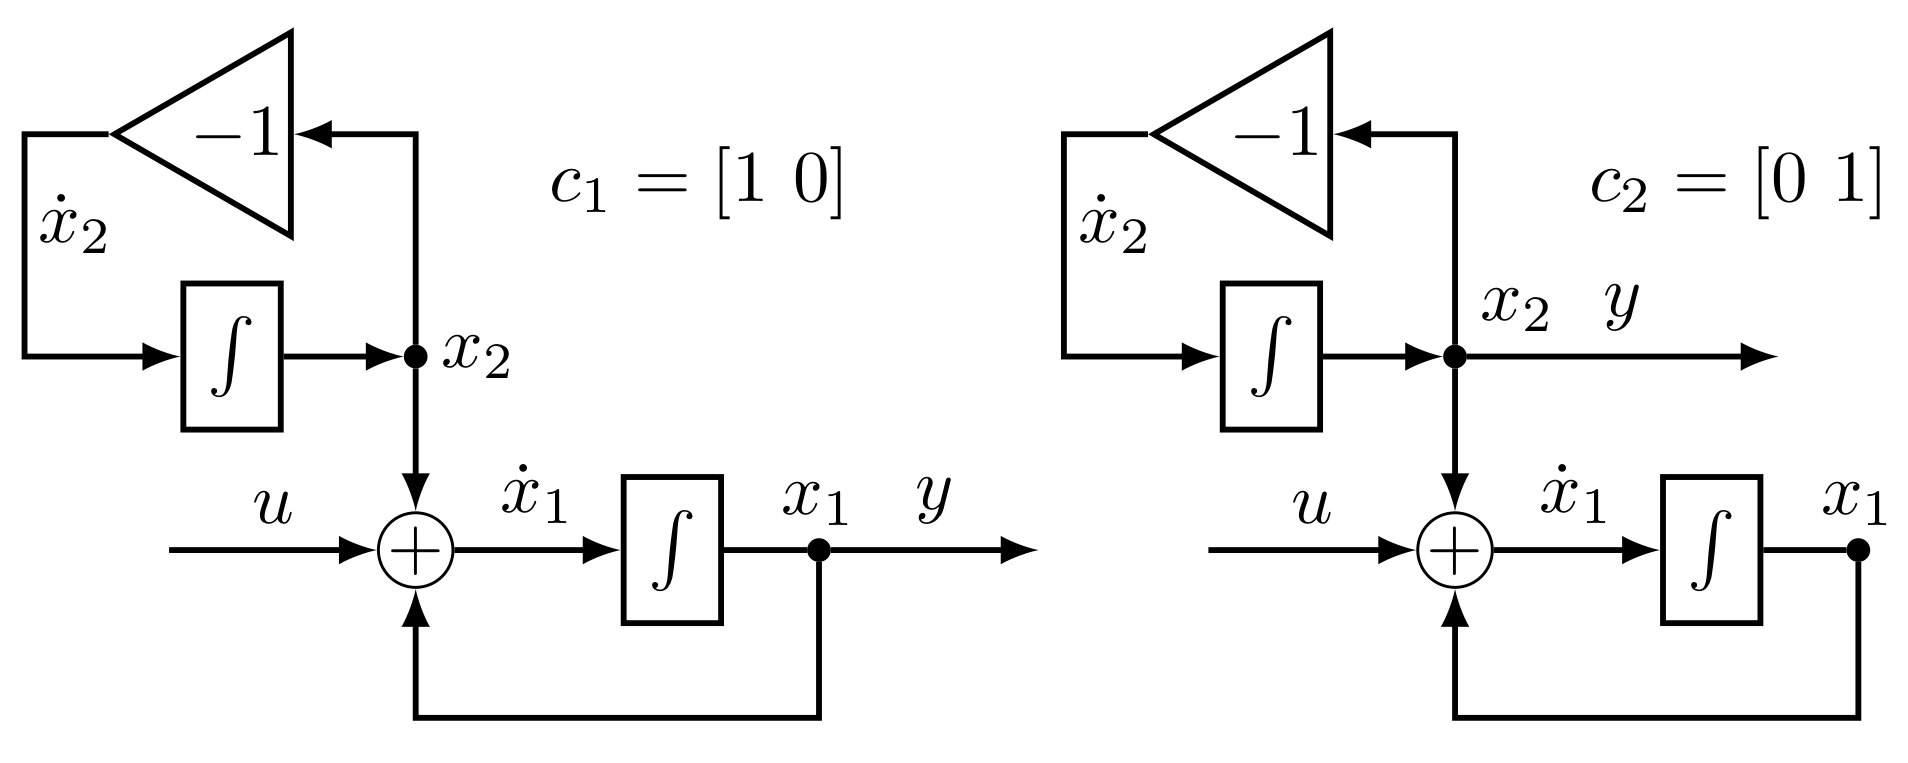
\includegraphics[width=0.6\linewidth]{03/graphisch.jpeg}
            \end{center}
        \subsubsection{Detektierbarkeit}
           Ein System ist nur detektierbar, falls all seine nicht-beobachtbaren Zustände asymptotisch stabil sind.
           
           \textit{Remarks:}
           \\Detectability is a weaker condition than observability.
           \\An (unstable) system is stabilizable, if the system is potentially stabilizable \textit{and} detectable.
            
        \subsection{Koordinatentransformationen} Ein Zustandsraum mit Koordinaten $x$ kann durch eine Koordinatentransformation in anderen Koordinaten $\tilde{x}$ beschrieben werden.
        \[ x(t) = T \cdot \tilde{x}(t) \hspace{10mm} T \in\mathbb{R}^{n\times n}, det(T)\neq0\]
        \[\frac{d}{dt}\tilde{x}(t) = T^{-1} \cdot A\cdot T \cdot \tilde{x}(t) + T^{-1} \cdot b \cdot u(t)\]
        \[y(t) = c\cdot T \cdot \tilde{x}(t) + d \cdot u(t)\]
        
        Fundamentale Systemeigenschaften  (Stabilität, Steuerbarkeit, Beobachtbarkeit, I/O-Verhalten) sind Transformationsinvariant.
\vfill\null\columnbreak        
        \subsection{Input/Output (I/O) Darstellung}
            Eine Zustandsraumdarstellung $\{A,b,c,d\}$ beschreibt das gesamte System (Zustände $x(t)$ und Ausgang $y(t)$ für gegebene $x(0) \& u(t)$). Oftmals ist man aber nur am I/O Zusammenhang $u(t) \rightarrow y(t)$ interessiert.\\\\
            \textbf{I/O-Beschreibung:}
            \begin{center}
                $\displaystyle y^{(n)}(t)+a_{n-1}\cdot y^{(n-1)}(t)+\dots+a_1\cdot y^{(1)}(t)+a_0\cdot y(t) = b_m\cdot u^{(m)}(t)+\dots+b_1\cdot u^{(1)}(t)+b_0\cdot u(t)$
            \end{center}
            
        
        \subsection{Zustandsraum Normalformen}
            Zustandsraumdarstellungen, welche sich für Analyse-Methoden besonders eignen, sind Normalformen oder eine kanonische Form.
            
            Eine wichtige Normalform ist die \textbf{Reglernormalform}.
            \begin{center}
               \[\left[{\renewcommand{\arraystretch}{1.3}\begin{array}{c|c}
              A & b\\
            \hline
            c & d
            \end{array}}
               \right]= \left[{\renewcommand{\arraystretch}{1.4}\begin{array}{ccccc|c}
               0 & 1 & 0 & \cdots & 0 & 0 \\
               0 & 0 & 1 &\ddots & \vdots & \vdots\\
            \cdots & \cdots & \cdots & \ddots & \vdots & \vdots \\
            0 & 0 & 0 & \cdots & 1 & 0\\
            -a_0 & -a_1 & -a_2 & \cdots & -a_{n-1} & 1 \\
            \hline
            b_0 & \cdots & b_m & 0 & \cdots & d
               \end{array}}
             \right]
               \] 
            \end{center}
            wobei $a_i,b_j$ aus der I/O-Darstellung oder aus $\Sigma(s)$ kommen:
            \[\Sigma(s) =\frac{b_ms^m+\dots+b_3s^3+b_2s^2+b_1s+b_0}{s^n+a_{n-1}s^{n-1}+\dots+a_3s^3+a_2s^2+a_1s+a_0}+d\]
        \subsection{Zustandsraumzerlegung}
            Die Sets von erreichbaren ($\mathcal{R}$) und/oder beobachtbaren ($\mathcal{O}$) Punkten sind \textbf{invariante Unterräume} im Zustandsraum. durch eine geeignete Koordinatentransformation $x = T\cdot\tilde{x}$ kann der gesamte Zustandsraum in die invarianten Unterräume $\{\tilde{x}_1,\tilde{x}_2,\tilde{x}_3,\tilde{x}_4\}$ zerlegt werden:
            Für die Beschreibung des I/O-Verhaltens ist also nur der Zustand $\tilde{x}_3$ relevant, da er der einzige ist, der gleichzeitig beobachtbar UND steuerbar ist. Die Anzahl Zustände $n$ im Unterraum $\tilde{x}_3$ entspricht der minimalen Anzahl Zustände, die zur Beschreibung des I/O-Verhaltens nötig sind. Deshalb wird die Darstellung des Systems in den Koordinaten $\tilde{x}_3$ \textbf{minimale Zustandsraumdarstellung} genannt:
            \begin{center}
                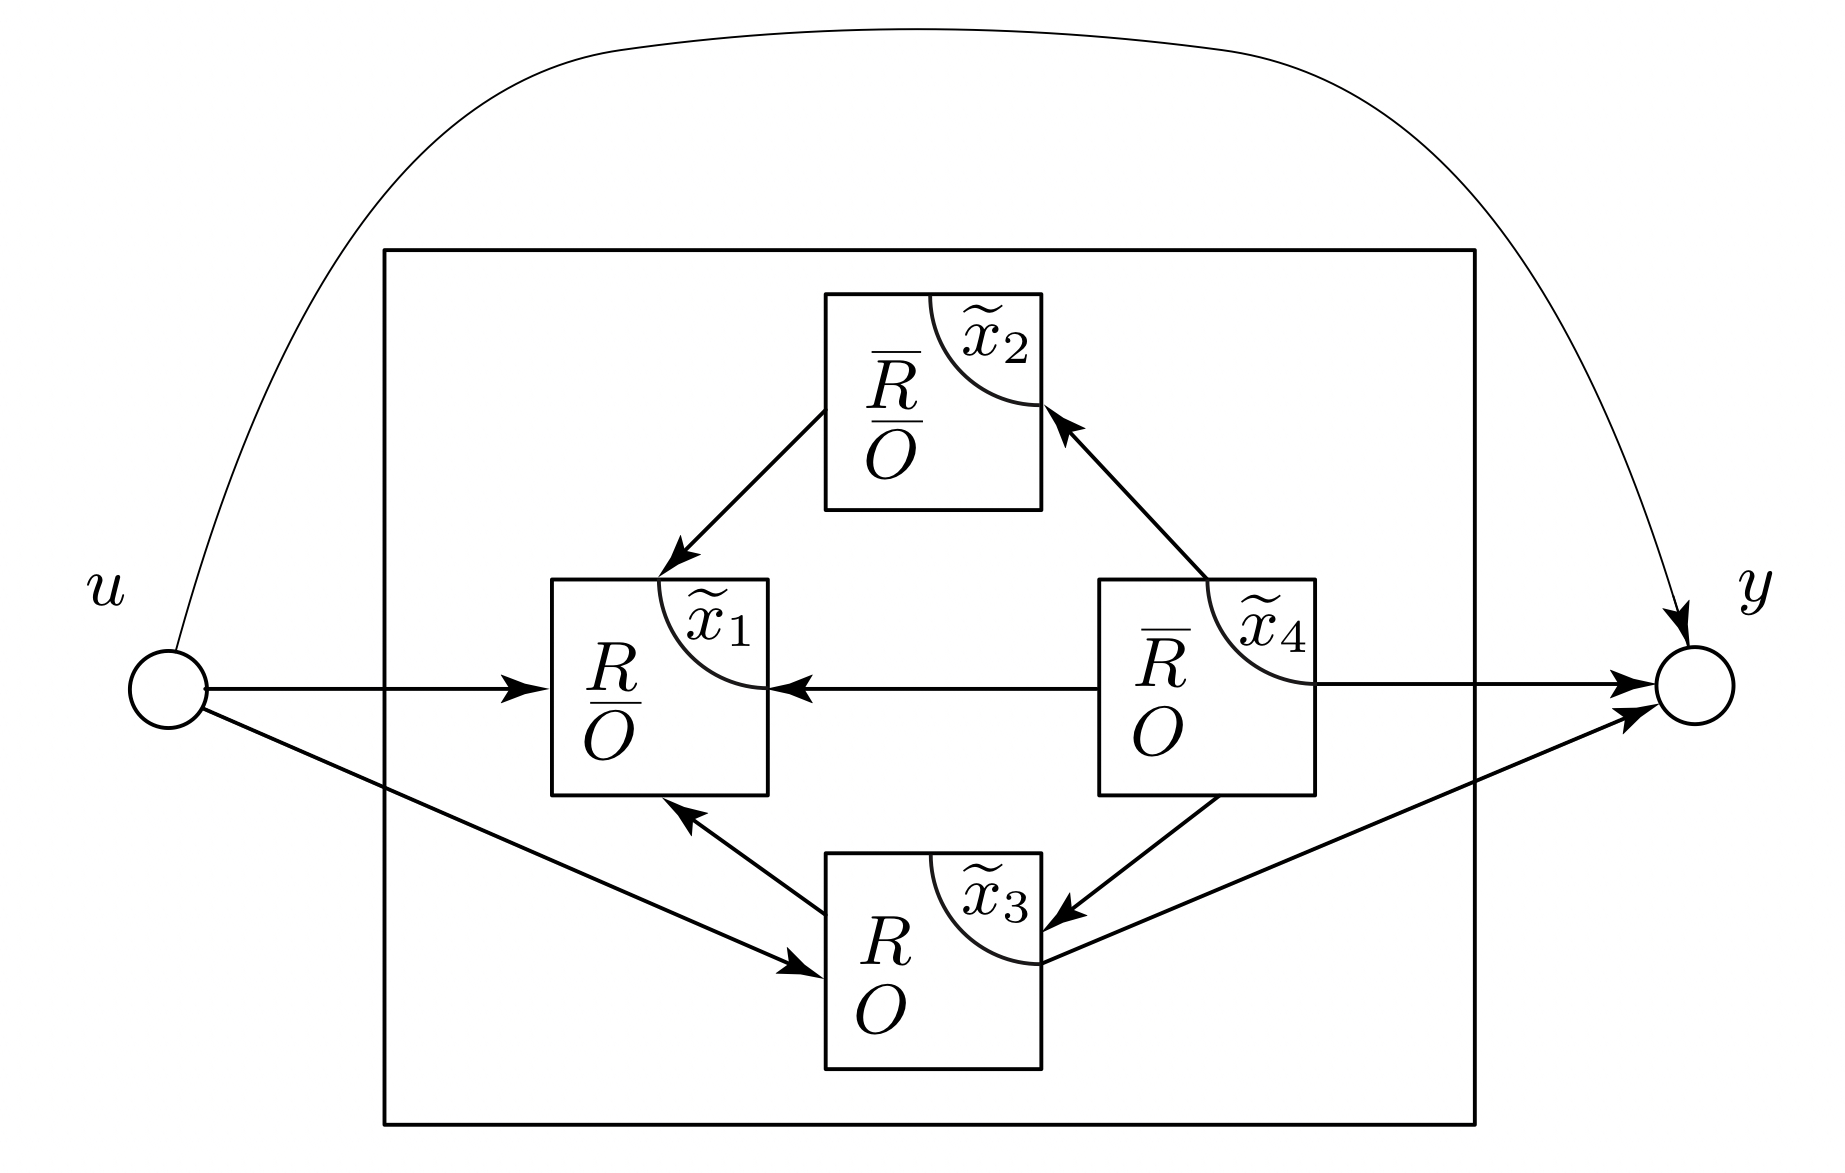
\includegraphics[width=0.4\linewidth]{03/invarianten.jpeg}
                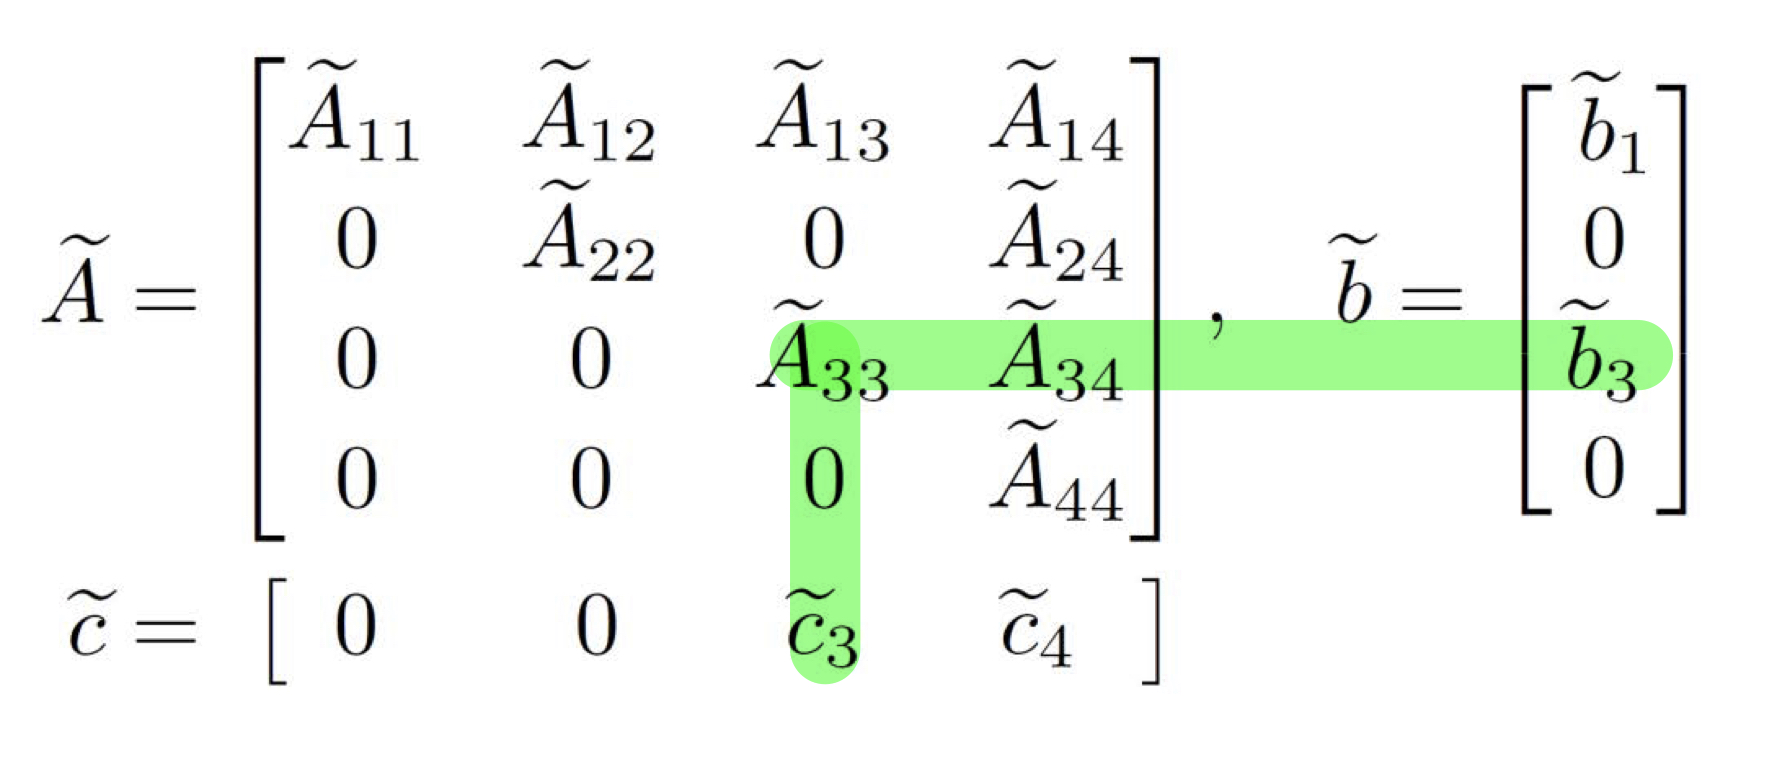
\includegraphics[width=0.5\linewidth]{03/minimal.jpeg}
                \\minimal realization $\rightarrow\{\tilde{A}_{33},\tilde{b}_3,\tilde{c}_3,d\}$ 
            \end{center}
            Vollständig steuerbar und beobachtbar (falls keine Pol-NST-Kürzung möglich, ist das System bereits in minimaler Form).
            % direkt Aus Systemmatrizen auslesen oder in Übertragungsfunktionsform $\Sigma(s)$ bringen und in Reglernormalform rücktransformieren. 
            
        \subsubsection{Bsp}
            Bestimme ob $\{A,b\}$ steuerbar ist, ohne $\mathcal{R}$ zu berechnen.
            \[ A=
            \begin{bmatrix}
            -1  &   -2  &   0\\
            -2  &  -1  &   0\\
            0   &   0   &   -2\\
            \end{bmatrix},
            b=
            \begin{bmatrix}
            1\\ 1\\ 1\\
            \end{bmatrix}
            \]
            \[\Downarrow diagonalisieren\quad \dot{\Tilde{x}}=D\cdot\Tilde{x}+V^{-1}\cdot b\cdot u\]
            \[
            \begin{bmatrix}
                \dot{\Tilde{x}}_1\\
                \dot{\Tilde{x}}_2\\
                \dot{\Tilde{x}}_3\\
            \end{bmatrix}
            =
            \begin{bmatrix}
            -3  &   0   &   0\\
            0   &   -2  &   0\\
            0   &   0   &   1\\
            \end{bmatrix}
            \cdot
            \begin{bmatrix}
                \Tilde{x}_1\\
                \Tilde{x}_2\\
                \Tilde{x}_3\\
            \end{bmatrix}
            +
            \begin{bmatrix}
            \sqrt{2}\\
            1\\
            0\\
            \end{bmatrix}
            \cdot
            u
            \]
            %$D$: Matrix mit diag($\lambda_i$) \& $V$ Matrix mit Eigenvektoren.\\
            System hat einen Zustand $\Tilde{x}_3$, der instabil ($\lambda_3=1$) \& nicht steuerbar ist.
            %\vfill\null